\newpage
\clearpage
\section{Introdução}


A era da Inteligência Artificial generativa marca um momento transformador na tecnologia, onde máquinas são capazes de criar conteúdos complexos e originais, desde textos e imagens até músicas e vídeos, com uma sofisticação sem precedentes. Esse avanço é impulsionado por modelos de aprendizado profundo que conseguem entender e replicar padrões de linguagem e dados de uma forma que simula a criatividade humana. Tecnologias de \textit{Large Language Models} (LLM) como Gemini \cite{geminiteam2024gemini}, LLama \cite{llama3blog} e ChatGPT \cite{Liu_2023} demonstram o potencial vasto dessa nova era, possibilitando aplicações inovadoras em diversas áreas, incluindo comunicação, entretenimento, educação e negócios. Essa evolução não só redefine a maneira como interagimos com a tecnologia, mas também levanta questões importantes sobre ética, privacidade e o futuro do trabalho.

O avanço da tecnologia no contexto da geração de texto e imagens se deve ao progresso significativo nos estudos de modelos de linguagem, combinado com o aumento exponencial do poder computacional necessário para treinar esses modelos. Nos últimos anos, o desenvolvimento de arquiteturas avançadas de redes neurais, como transformadores, tem permitido a criação de modelos de linguagem cada vez mais sofisticados e precisos, capazes de entender e gerar conteúdo com alta qualidade e coerência.

Esses avanços foram catalisados por inovações como o modelo GPT (\textit{Generative Pre-trained Transformer}), que utiliza grandes quantidades de dados textuais para aprender padrões e nuances da linguagem humana. Paralelamente, o poder computacional necessário para treinar esses modelos aumentou significativamente, com o uso de GPUs (unidades de processamento gráfico) e TPUs (unidades de processamento de tensor) de alta performance, permitindo que redes neurais cada vez maiores e mais complexas sejam treinadas em prazos razoáveis \cite{wang2019benchmarkingtpugpucpu}.

Além disso, o surgimento de novas técnicas de otimização e algoritmos de aprendizado profundo, tem contribuído para a eficiência e eficácia desses modelos. Essas melhorias tecnológicas não apenas elevaram o nível de sofisticação dos modelos de IA generativa, mas também ampliaram seu campo de aplicação, permitindo avanços em áreas como tradução automática, criação de conteúdo, design gráfico, e até mesmo no desenvolvimento de novas formas de arte e entretenimento.

O impacto dessas inovações é profundo e abrangente, transformando setores industriais inteiros e remodelando a forma como interagimos com a informação e a tecnologia. No entanto, esses avanços também trazem desafios significativos, incluindo questões de ética e privacidade, a necessidade de regulamentação adequada, e a importância de garantir que essas tecnologias sejam utilizadas de maneira responsável e inclusiva. 

O \textit{Retrieval Augmented Generation} (RAG) \cite{gao2024retrievalaugmentedgenerationlargelanguage} é um processo avançado de geração de texto que capacita modelos a produzir conteúdo a partir de uma combinação de geração baseada em aprendizado profundo e recuperação de informações relevantes de bases de dados extensas e externas às utilizadas para o treinamento do LLM. Esse método funciona integrando mecanismos de busca que recuperam dados pertinentes ao contexto ou ao tema solicitado, que são então utilizados pelo modelo de geração para criar textos mais informativos, precisos e contextualizados.

O RAG é especialmente eficaz em tarefas que exigem conhecimento atualizado ou especializado, pois permite ao modelo acessar e incorporar informações recentes e específicas diretamente de fontes confiáveis. Isso melhora significativamente a qualidade e a relevância do texto gerado, superando as limitações dos modelos puramente generativos que dependem exclusivamente do conhecimento armazenado durante o treinamento. Além disso, essa abordagem pode ser adaptada para uma ampla variedade de aplicações, desde assistentes virtuais que fornecem respostas detalhadas e precisas até sistemas de suporte ao cliente que oferecem soluções informadas e contextualmente apropriadas.

Desde 2020 o modelo GPT vem sido evoluido para o contexto RAG, através de diversas técnicas que compoem a estrutrutura de Pré-Treino, Fine-Tuning e a forma de fazer inferencia neses modelos. Técnicas avançadas como Re-Ranker, tem como objetivo otimizar as respostas e gerar textos cada vez mais assertivos de acordo com a pergunta feita.
A Figura \ref{fig:rag1} representa o avanço das tecnologias utilizadas pelo GPT \cite{Liu_2023} no contexto RAG ao longo dos anos

\begin{figure}[H]
    \centering
    \caption{Avanço de tecnologias do contexto RAG ao longo dos anos}
    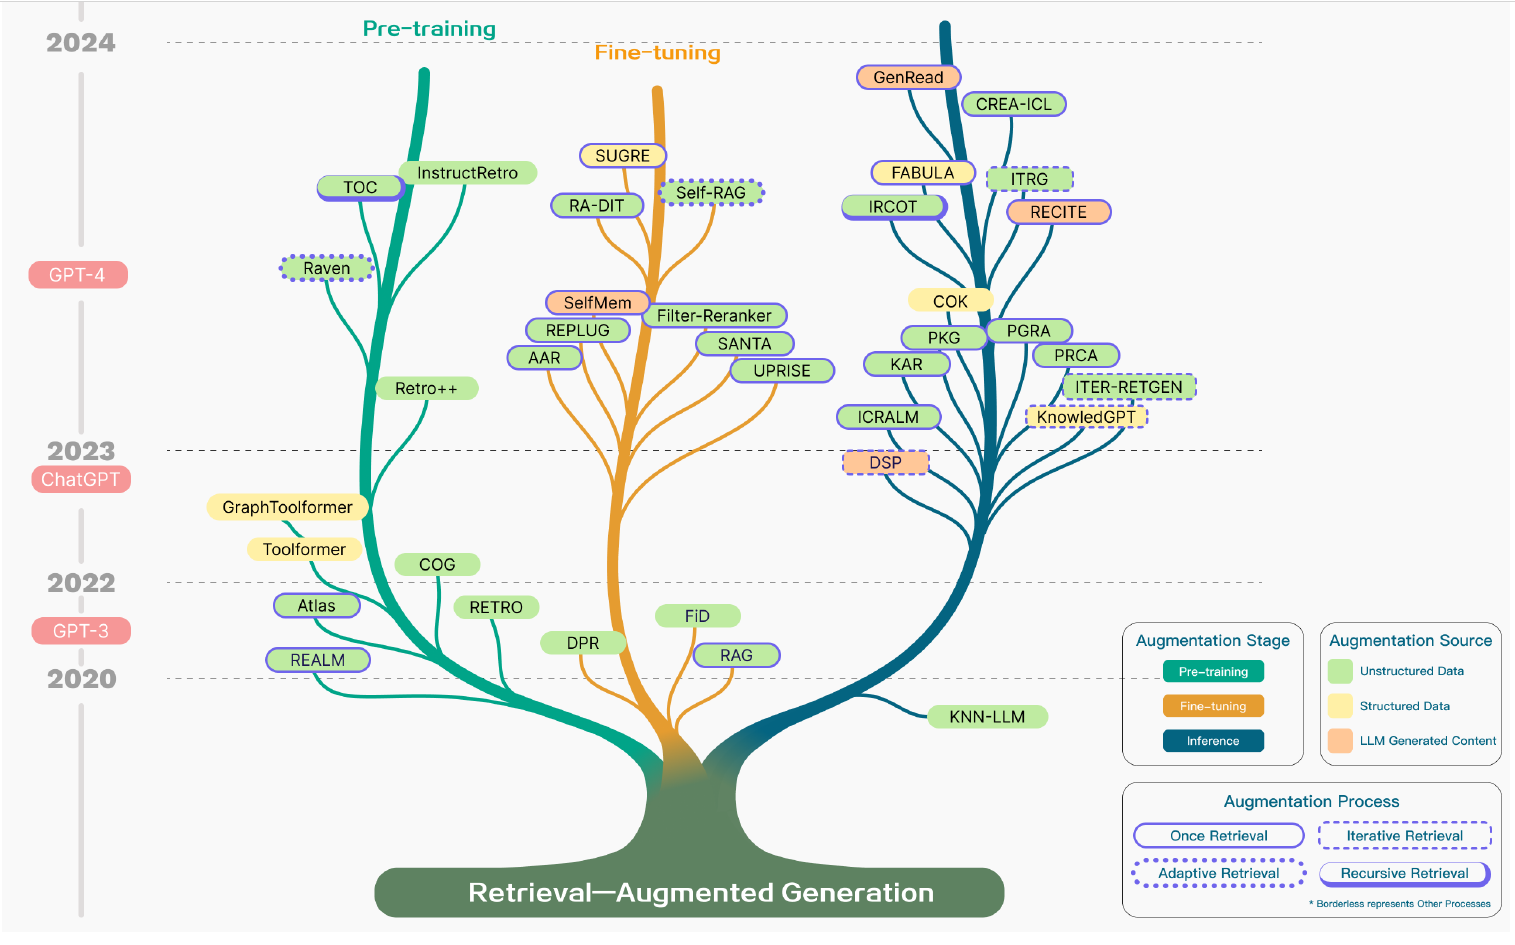
\includegraphics[width=\linewidth]{img/RAG/rag1.png}
    \caption*{Fonte: \cite{gao2024retrievalaugmentedgenerationlargelanguage}}
    \label{fig:rag1}
\end{figure}

A implementação de um \textit{pipeline} de Recuperação de Informação com RAG é essencial para otimizar a gestão de documentos e a recuperação de informações em diversos contextos empresariais e organizacionais. Esse fluxo começa com a recuperação de informações, onde técnicas avançadas de busca e indexação localizam dados relevantes a partir de grandes repositórios de informações estruturadas e não estruturadas. Em seguida, esses dados são processados por modelos de geração de texto que sintetizam a informação recuperada, produzindo respostas ou relatórios detalhados e contextualmente apropriados. Por exemplo, no atendimento ao cliente, o RAG pode fornecer respostas imediatas e precisas a consultas complexas, melhorando significativamente a experiência do usuário e reduzindo o tempo de espera. Em contextos corporativos, como financeiro ou jurídico, o \textit{pipeline} pode automatizar a extração de informações críticas e a geração de relatórios customizados, adaptando-se às necessidades específicas de cada situação. A personalização é um aspecto vital, permitindo que o RAG atenda a diferentes departamentos dentro de uma organização, enquanto sua escalabilidade possibilita a aplicação tanto em pequenas empresas quanto em grandes corporações. Além disso, a automação proporcionada pelo RAG minimiza erros humanos e aumenta a precisão dos dados, crucial em áreas sensíveis como saúde e governança. Com sua capacidade de inovar e melhorar a eficiência operacional, o RAG posiciona a organização de maneira competitiva no mercado, demonstrando um compromisso com a modernização e a excelência na gestão de informações. 
A Figura \ref{fig:rag12} representa o fluxo essencial de RAG. 

\begin{figure}[H]
    \centering
    \caption{Fluxo e etapas de Retrieval-Augmented-Generation}
    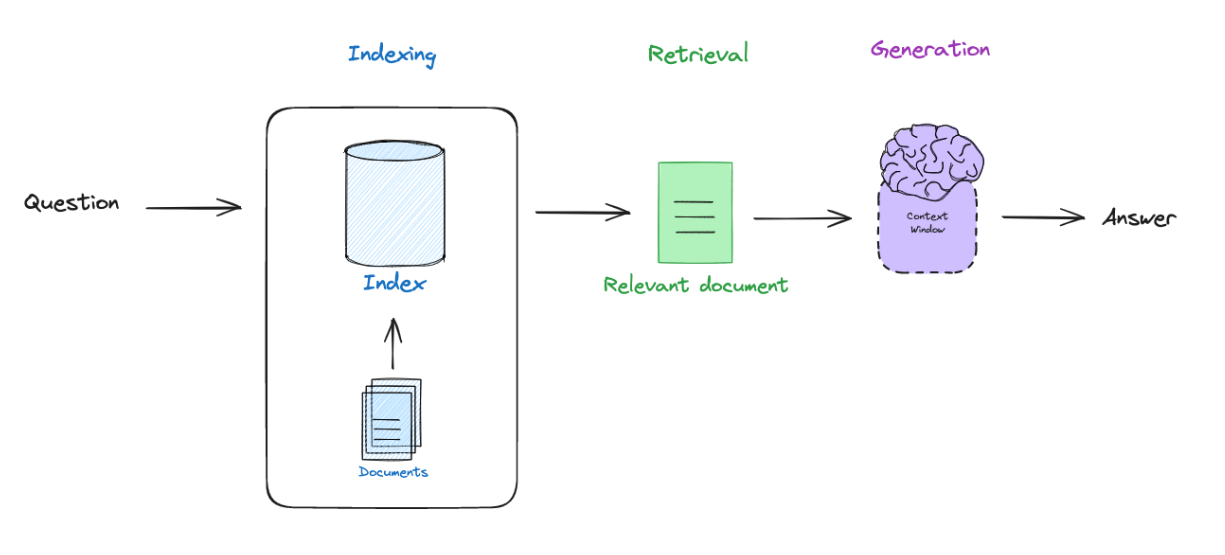
\includegraphics[width=\linewidth]{img/RAG/RAG2.png}
    \caption*{Fonte: \cite{SlidesMartin}}
    \label{fig:rag12}
\end{figure}

 Um dos métodos para o ranqueamento de documentos dentro desse contexto é o BM25 \cite{10.1145/2682862.2682863}, uma variante do modelo de espaço vetorial que utiliza a frequência dos termos para avaliar a relevância dos documentos em relação a uma consulta. O BM25, ou \textit{Best Matching} 25, aplica uma fórmula probabilística que pondera a frequência dos termos e a normalização do comprimento do documento, permitindo um balanceamento eficiente entre a quantidade de termos correspondentes e a penalização de documentos excessivamente longos. Ao integrar o BM25 em um pipeline de RAG, é possível selecionar os documentos mais relevantes de um grande repositório de dados, garantindo que o modelo de geração de texto receba as informações mais pertinentes para criar respostas precisas e contextualmente adequadas. Dessa forma, a combinação de BM25 com a geração automatizada potencializa a eficiência e a precisão dos sistemas de perguntas e respostas, tornando-os extremamente valiosos em contextos dinâmicos onde a rapidez e a acurácia são cruciais.

Após a indexação e o ranqueamento dos documentos utilizando métodos como o BM25, o processo de Aumento em um sistema de RAG pode ser aprimorado através do \textit{fine-tuning} de modelos de linguagem pré-treinados, como GPT (\textit{Generative Pre-trained Transformer}) \cite{Liu_2023}, BERT \textit{(Bidirectional Encoder Representations from Transformers)} \cite{DBLP:journals/corr/abs-1810-04805} ou T5 \textit{(Text-to-Text Transfer Transformer}) \cite{2020t5}.

Na etapa de \textit{Augmentation}, \textit{fine-tuning} por sua vez, possibilita a geração de saídas mais estilizadas e personalizadas, adaptando-se a diferentes formatos de dados de entrada e demandando conteúdos específicos por meio de conjuntos de dados direcionados. A sinergia resultante do \textit{fine-tuning} conjunto de documentos previamente ranqueados e do \textit{Generation}, aumenta a capacidade de generalização do modelo, embora também aumente o consumo de recursos. 

Ao realizar o \textit{fine-tuning} desses modelos, estamos capacitando-os a compreenderem melhor a informação recuperada e a produzirem respostas de maior qualidade e relevância. Essa integração entre a informação dos documentos ranqueados e os modelos de geração de texto refinados através do \textit{fine-tuning} resulta em um processo mais eficaz e preciso em sistemas RAG, proporcionando respostas dinâmicas e personalizadas para diferentes necessidades e contextos. \cite{gao2024retrievalaugmentedgenerationlargelanguage}.

A Geração Aumentada por Recuperação, introduzida por Lewis \cite{lewis2021retrievalaugmented}, representa um marco na área de processamento de linguagem natural. Essa inovadora técnica combina a força de modelos de linguagem pré-treinados (LLMs) com a capacidade de busca de informações relevantes, transcendendo as limitações dos modelos tradicionais.

O RAG se diferencia pela utilização de memórias paramétrica e não paramétrica. A memória paramétrica, geralmente um modelo LLM (\textit{Large Language Model}) pré-treinado, fornece a base para a geração de texto. Já a memória não paramétrica, como um índice vetorial denso ou esparso de dados de um determinado contexto, atua como um repositório de informações externas. A chave reside na integração dessas duas memórias através de um modelo de recuperação pré-treinado.

Em resumo, o RAG funciona como um sistema híbrido que combina a busca por informações com a geração de texto. Através de um mecanismo de recuperação, o modelo extrai as partes mais relevantes de documentos relevantes de um extenso corpus. Na sequência, essas informações extraídas são utilizadas por um LLM para gerar respostas precisas e informativas.

O objetivo desta monografia é realizar um levantamento das técnicas para a construção e abordagem de um fluxo RAG (Retrieval-Augmented Generation), detalhando métodos adequados para cada etapa, como Recuperação (\textit{Retrieval}), Aumento (\textit{Augmentation}) e Geração (\textit{Generation}). Além disso, serão exploradas as variantes de abordagens utilizadas para aprimorar o fluxo de RAG como um todo.

Essa monografia abordará a visão geral de um \textit{Transformer} e sua relação com os \textit{Large-Language-Models}, seguido do detalhamento dos modelos BERT e LLama3, que podem ser utilizados e adaptados para as etapas de \textit{Retrieval}, \textit{Augmentation} e \textit{Generation}, e por fim o detalhamento de todo o fluxo de RAG e as formas de realizar a etapa de Retrieval.